\documentclass{article}

\usepackage[T1]{fontenc}
\usepackage[utf8]{inputenc}
\usepackage[english,french]{babel}
\usepackage{graphicx}
\usepackage{incgraph,tikz}

\newcommand{\VSpace}{\vspace{1.5cm}}
\newcommand{\HRule}{\rule{\linewidth}{0.5mm}}

\begin{document}
\begin{titlepage}
    \begin{sffamily}
        \begin{center}
        
            
\includegraphics[scale=0.3]{images/LOGO ST.png}~\\
            \VSpace
            \textsc{\LARGE UFR Sciences et Technique BESANCON}\\
            \vspace{0.5cm}
            \textsc{\Large Rapport de Projet Licence 3 informatique}\\
            \VSpace
            \HRule\\{\huge\bfseries  Création d'un jeu d'infiltration\\}
            \HRule\\
            \VSpace
            \textsc{image KGB}
            \VSpace
    
            \begin{minipage}{0.5\textwidth}
              \begin{flushleft} \large
                \textsc{Mathieu} BART\\
                \textsc{Florian} WIEDENKELLER\\
                \textsc{Jérémy} BATTAGLIA\\
                
              \end{flushleft}
            \end{minipage}
            \begin{minipage}{0.4\textwidth}
              \begin{flushright} \large
                \emph{Tuteur :} M. \textsc{Julien} BERNARD\\
              \end{flushright}
            \end{minipage}
            \vfill
        
            {\large Promotion 2019-2020}
        \end{center}
    \end{sffamily}
\end{titlepage}

\newpage
\hypersetup{pdfborder=0 0 0}

\renewcommand{\contentsname}{Sommaire}

\tableofcontents

\vspace*{\stretch{1}}
\section{Introduction}

Notre projet est de programmer un jeu d'infiltration en utilisant le framework\footnote{Un framework désigne un ensemble cohérent de composants logiciels structurels, qui sert à créer les fondations ainsi que les grandes lignes de tout ou d’une partie d'un logiciel.}
C++ Gamedev Framework (GF). Un jeu d'infiltration est un jeu dans lequel le joueur a différents objectifs à accomplir. Il doit les accomplir sans se faire repérer sinon il pourrait perdre la partie.  Nous pouvions nous inspirer du jeu : \textit{Commandos, derrière les lignes ennemis}, cependant nous avons préféré utiliser notre imagination pour ce qui concerne l'histoire ou les objectifs du jeu.\bigbreak
Le joueur incarnera donc un bébé qui souhaite s'échapper d'une \og garderie\fg. Pour que le joueur s'échappe, il aura besoin de trouver une clef qui apparaîtra aléatoirement dans le niveau à chaque nouvelle partie. Une fois la clef récupérée, il pourra partir de la garderie via la grille que le joueur verra au début du jeu en la touchant. Cependant des gardes surveillent les couloirs de cette garderie, et si l'un d'entre eux à le malheur de voir le joueur, alors il perdra directement. 


\newpage

\section{Présentation du jeu}
\subsection{But et fonctionnement}
Comme dit précédemment le joueur incarne un bébé souhaitant s'échapper d'une \og garderie\fg pour cela il doit se déplacer à l'aide des flèches directionnelles ou des touches \textbf{ZQSD} respectivement pour haut, gauche, bas et droite afin de récupérer une clef et de retrouver la sortie tout en évitant les geôliers.\bigbreak
La clef recherchée pour s'échapper de cet endroit peut apparaître à différents endroits afin que deux parties puissent être différentes l'une de l'autre. Il faut donc explorer les différentes pièces et traverser les différents couloirs à la recherche de cette clef. Une fois celle-ci acquise, le joueur devra rejoindre la sortie afin de s'enfuir.\bigbreak
Néanmoins durant son exploration des lieux le joueur sera gêné par les gardiens de l'endroit. Ces gardes ont pour ordre d'éliminer le bébé à vue il faut donc à tout prix éviter leur regard et leur contact ! Ils se déplacent en suivant un pattern mais certains peuvent se tourner de façon irrégulière.\bigbreak
Enfin pour aider le joueur au cours de son échappatoire il pourra trouver des bonus sous forme de couche. Certaines permettent de passer inaperçu tandis que d'autre font accélérer le bébé. Pour les utiliser appuyer sur les boutons gauche et droit de la souris respectivement pour le bonus de rapidité et celui d'invisibilité.\bigbreak

\subsection{Diagramme de classe}


\section{Outils et choix technologiques}
Notre sujet nous imposait un développement en \textbf{C++} en utilisant le framework \textbf{Gamedev Framework} développé par \textbf{Julien BERNARD}. En parallèle de celui-ci et afin de gérer les collisions nous avions deux options:
\begin{itemize}
    \item Créer et implémenter nous même des fonctions de détection et de gestion des collisions.
    \item Utiliser un moteur physique déjà existant et l'adapter à nos besoins.
\end{itemize}\bigbreak
Chacune des options possède des avantages et des inconvénients. Pour la première cela nous permettrais de savoir exactement comment sont gérés nos collisions et de ne développer que ce dont nous avons besoin mais celle-ci aurait pu être très chronophage c'est pourquoi nous avons choisie la deuxième solution. Le moteur physique \textbf{Box2D} développé par \textbf{Erin Catto} nous permettait de facilement gérer les collisions entre nos objets une fois ceux-ci relié à un \textbf{b2Body}. La difficulté avec Box2D était justement cette liaison entre notre objet et la représentation de box2D mais un autre avantage de box2D était la documentation que l'on pouvait trouver sur internet afin de nous aider à l'utiliser.\bigbreak
Pour ce qui est de la gestion des images et animations nous avons utilisés les fonctions de GF qui étaient simple d'utilisation. Afin de créer la carte nous avons utilisé le logiciel \textbf{Tiled} permettant de créer des cartes à partir de set de tuiles existant. Enfin pour l'ambiance sonore du jeu nous avons utilisé la partie audio de \textbf{SFML} (Simple and Fast Multimedia Library).

\subsection{SFML}
SFML est une bibliothèque destinée à la création de programmes interactifs (principalement des jeux vidéo compris) en C++. Elle permet de gérer les aspects multimédia de ces programmes incluant donc l'image comme le son. Dans notre projet nous avons utilisé la partie audio de SFML qui fournit deux classes à cet effet : \textbf{sf::Sound} et \textbf{sf::Music}. Cela nous a permis d'intégrer au jeu une musique, des sons d'ambiance comme le bruit des pas du bébé, des dialogues oraux durant l'introduction et quelques bruitage pour les bonus. SMFL s'adaptait à nos besoins et les inconvénients possible de cette bibliothèque ne nous affectait pas, par exemple SFML possède une limite interne limitant le nombre de son pouvant être jouer en même temps (cette limite étant dépendante du système d'exploitation et généralement d'une valeur de 256 sons).

\subsection{Tiles}
Tiles est un logiciel d'édition de carte 2D. Celui-ci permet à partir d'un set de tuile de créer une carte 
\subsection{Box2D}
\subsection{GF}

\newpage

\section{Développement du jeu}
 
\subsection{Gestion des entités}

GF et Box2D sont deux Frameworks qui possèdent leur propre type d'entité pour représenter des objets, l'entité de GF a des caractéristiques propices à l'affichage tandis que l'entité de Box2D se spécialise dans la gestion des collisions. Cela implique donc que leurs classes possèdent des paramètres différents et n'ont pas la même utilité dans leur Framework respectif. Pourtant chaque entité que nous avons créé doit se comporter comme des entités de GF et de Box2D afin d'associer leurs avantages.\\

Nous avons fait hérité nos entités de la classe Entity de GF pour avoir accès aux fonctions \og \textit{render}\fg et \og \textit{update}\fg. Elles sont des fonctions virtuelles à implémenter pour nos objets, avec \og \textit{render}\fg nous affichons la représentation graphique de notre objet, celle-ci pouvant changer si c'est un objet avec plusieurs animations, tandis qu'avec la fonction \og \textit{update} nous gérons toutes les modifications de variables qui interagissent avec le temps, par exemple une mise-à-jour de la position d'un objet qui se déplace. C'est lors de l'initialisation de l'objet que nous donnons les différents paramètres qui définiront l'objet, sa position, son visuel, etc.\\

Pour autant, la gestion de la physique de notre jeu est géré par Box2D. Pour intégrer les différents calculs de collision, nos entités possèdent un paramètre particulier : un \og \textit{b2Body}\fg. Ce paramètre permet de lier notre entité avec un objet utilisable et gérable par Box2D. Ce paramètre possède ce qu'on appelle une \og \textit{b2Fixture}\fg qui donne plusieurs options pour la gestion des collisions, comme par exemple des filtres de collision ou encore des ajouts de variables utilisateurs. La b2Fixture est donc un élément important pour les collisions entre les différents \og \textit{b2Body}\fg de Box2D. L'attribution des \og \textit{b2Body}\fg est faite à part dans un classe dédiée à la gestion de la Physique du jeu : \og \textit{Physics}\fg. Cette classe contient pratiquement toutes les informations du jeu liées à Box2D.\\

En synchronisant les informations de notre entité avec celle de l'objet \og \textit{b2Body}\fg, nous avons des objets qui sont affichés sur notre écran de jeu et possèdent un corps physique les empêchant de traverser les autres.

\subsubsection{Gestion des déplacements}
Pour les déplacements du bébé ils sont mis à jour en fonction du choix de déplacement fait par le joueur grâce à la détection des touches au travers d'action définies. 

Un déplacement est un ensemble constitué d'une position, d'une vélocité et d'une vitesse, si le joueur va dans une direction il accélère jusqu'à atteindre une vitesse maximale et quand le joueur change de direction ça vitesse revient à l'état de départ avant d'augmenter à nouveau et ainsi de suite de manière à donner un petit effet d'accélération/décélération. La direction d'une entité est définie grâce à sa vélocité par rapport à un axe x et un axe y ayant pour origine le coin supérieur gauche de la fenêtre. Il s'agit donc d'un vecteur composé de deux float l'un permettant de définir le déplacement sur l'axe des abscisses et l'autre celui sur l'axe des ordonnées. De ce fait un personnage ayant une vélocité de 50,-50 se déplacera vers le haut et vers la droite.
Enfin la position du bébé est mise à jour à chaque update ainsi que son animation en fonction de l'orientation du bébé.\bigbreak
Pour le cas des ennemies il s'agit de mouvement prédéfinis. Chaque ennemie est initialisé à une position définie avec une vitesse, une orientation, un type de trajet et une distance à parcourir. Grâce à ces informations nous allons pouvoir actualiser son orientation et sa position. Prenons l'exemple d'un ennemie faisant des aller-retour dans un couloir. 

    \begin{figure}[ht]
        \begin{center}
            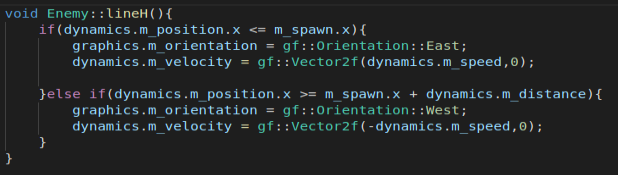
\includegraphics[width=1\textwidth]{images/screen_dep_ligne.png} 
        \end{center}
        \caption{Fonction de déplacement en ligne horizontale}
        \label{screen_fct_dep_ligne}
    \end{figure}

Comme nous pouvons le voir en Figure \ref{screen_fct_dep_ligne}, l'ennemie va changer son orientation en fonction de la distance qu'il a parcourue depuis son point d'apparition. En plus de changer l'animation nous allons aussi changer sa vélocité puisque la vélocité indique à l'entité dans quelle direction aller.\bigbreak
Ainsi nous avons initialiser 3 types de déplacements différents pour les ennemies:
    \begin{itemize}
        \item Les lignes horizontales.
        \item Les lignes verticales.
        \item Les rondes de garde se traduisant par le tracé d'un carré.
    \end{itemize}\bigbreak
Néanmoins un ennemie n'est pas forcer de se déplacer et peut être statique c'est pour cela que chaque ennemie à un attribut \textbf{STATUS} permettant de savoir s'il se déplace ou non. Les ennemies statiques ont pour particularité de changer d'orientation aléatoirement au bout de quelques secondes. Ceux-ci pouvant reprendre la même orientation plusieurs fois de suite, il est donc possible que leur orientation ne change pas toujours offrant une difficulté supplémentaire au joueur qui doit saisir le timing entre deux changement d'orientation.\bigbreak
Enfin, et ce pour le bébé comme pour les ennemies, la position du b2Body associé à chaque entité est mise à jour en fonction de la nouvelle position de l'objet.


\subsubsection{Messages}
Afin de détecter un évènement dans le jeu, comme le fait de ramasser la clef, de gagner ou encore de perdre nous utilisons les messages qui sont disponibles avec GF. Nous avons dans notre main, des handlers\footnote{Un handler est un module/fonction gérant une situation particulière comme une exception dans un processus.} pour chacun des messages. Ces différents messages sont définis dans notre header \textbf{Messages}. Ceux-ci permettent de recevoir et d'interpréter le message reçu par le main. Par exemple pour le cas de la clef qui a été ramassé par le joueur, on envoie le message au moment où le joueur rentre en collision avec celle-ci. Quand le message est reçu par le main, nous sommes dans la capacité de changer des variables présentes dans le main. Quand le message de la clef est reçu, on peut grâce au message afficher sur l'écran un texte pour indiquer au joueur ce qu'il doit faire maintenant.


\subsubsection{Gestion des collisions}
Chaque mur et chaque personnage possède une hitbox. Une hitbox peut être nommé \og masque de collisions \fg en français. Elle sert à délimiter une zone sur un personnage pour détecter les collisions que ce personnage aura avec d'autres personnages ou le décor qui eux aussi ont leur propre hitbox. Suivant ce que nous voulons en faire nous pouvons définir des actions quand des hitboxs rentrent en collisions entre-elles. Vu que nous utilisons Box2D, nous définissons un corps de la façon suivant la figure :
\begin{figure}[ht]
    \begin{center}
    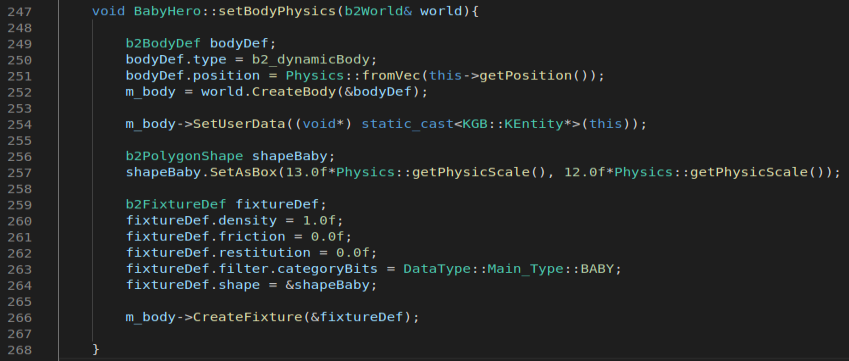
\includegraphics[scale=0.55]{images/creation_hitbox.PNG}
    \caption{Création d'une hitbox}
    \label{hitbox}
    \end{center}
\end{figure}
Le \texttt{\textbf{m\_body->setUserData(...)}} permet de définir le type d'entité afin de bien gérer les collisions plus tard. En effet, chacune des entités héritent de la même classe \textbf{KEntity}. Dans \textbf{KEntity}, nous avons une fonction \texttt{\textbf{getEntityType()}} qui renvoie un nombre différent suivant l'entité qui appel cette fonction (qui est redéfinie dans chaque entité). Ensuite, pour gérer correctement les collisions nous avons une classe \textbf{b2dContactListener} qui nous permet, suivant les deux entités qui rentrent en collisions, de faire un transtypage vers le type d'entité correspondant.
Une fois le cast effectué, nous appelons la fonction \texttt{\textbf{startContact(..)}} de chacune des entités afin de faire une action suivant avec qui cette entité est entré en collision. Vu que seulement la collision du bébé nous intéresse nous regardons avec qui il entre en collision.

\begin{figure}[ht]
    \begin{center}
    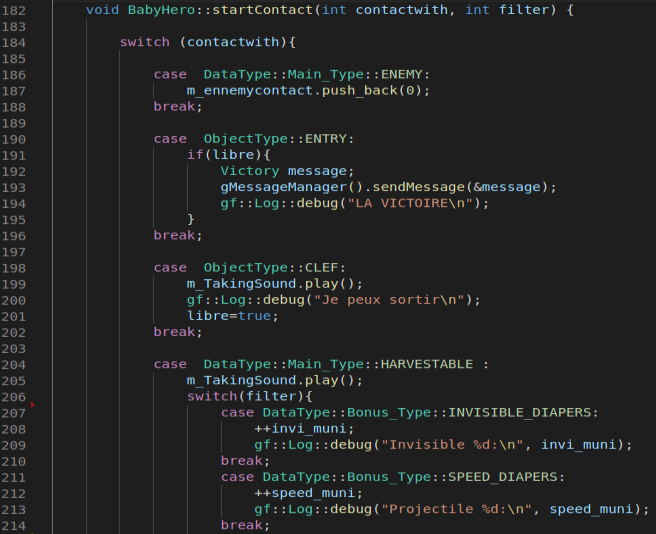
\includegraphics[scale=0.55]{images/baby_collisions.png}
    \caption{Actions d'une collision suivant l'entité}
    \label{baby_collisions} 
    \end{center}
\end{figure}

Nous avons donc un \textbf{switch} pour gérer les différents cas. On peut voir que si le bébé entre en collision avec la clef, cela envoie un message au main. On peut voir aussi qu'il est bien dans l'obligation de ramasser la clef avant de pouvoir envoyer le message de victoire car \textbf{libre} doit être \textbf{true}. Et c'est uniquement au moment où le joueur rentre en collision avec la clef que celui-ci peut donc en quelque sorte \og activer \fg l'action de collision avec \textbf{ObjectType::ENTRY}, qui est entre autre la grille que l'on voit au début.

\subsection{Création d'un niveau}
Pour créer un niveau, plus précisément une carte de jeu nous avons du dans un premier temps décider quel angle de vue allait avoir notre jeu. Nous pensions à une vue de dessus (dans le genre de \textit{Grand Theft Auto 1}) mais nous avons choisi une vue de dessus un peu différente (en 3/4) comme celle d'un jeu bien connu : \textit{The Legend Of Zelda}.\bigbreak Comme le but du projet est la programmation d'un jeu et celui de sa conception graphique, nous avons pris la liberté de prendre des ressources libres de droit disponibles sur internet. Ensuite il a fallu trouver un moyen de créer cette carte. Après quelques recherches sur ce qu'il se fait et des outils que nous avons à porté de main, nous avons décidé de faire une carte à la main à l'aide du logiciel \textbf{Tiled} avec les ressources trouvées sur internet. Cette carte est en format \textbf{.tmx} car GF prend en charge ce format. Donc avec un \textbf{tileset}, soit un ensemble de tiles -autrement dit de \og tuiles\fg- nous avons pu varier les tuiles utilisées dans la conception de la carte. 
\begin{figure}[ht]
    \begin{center}
    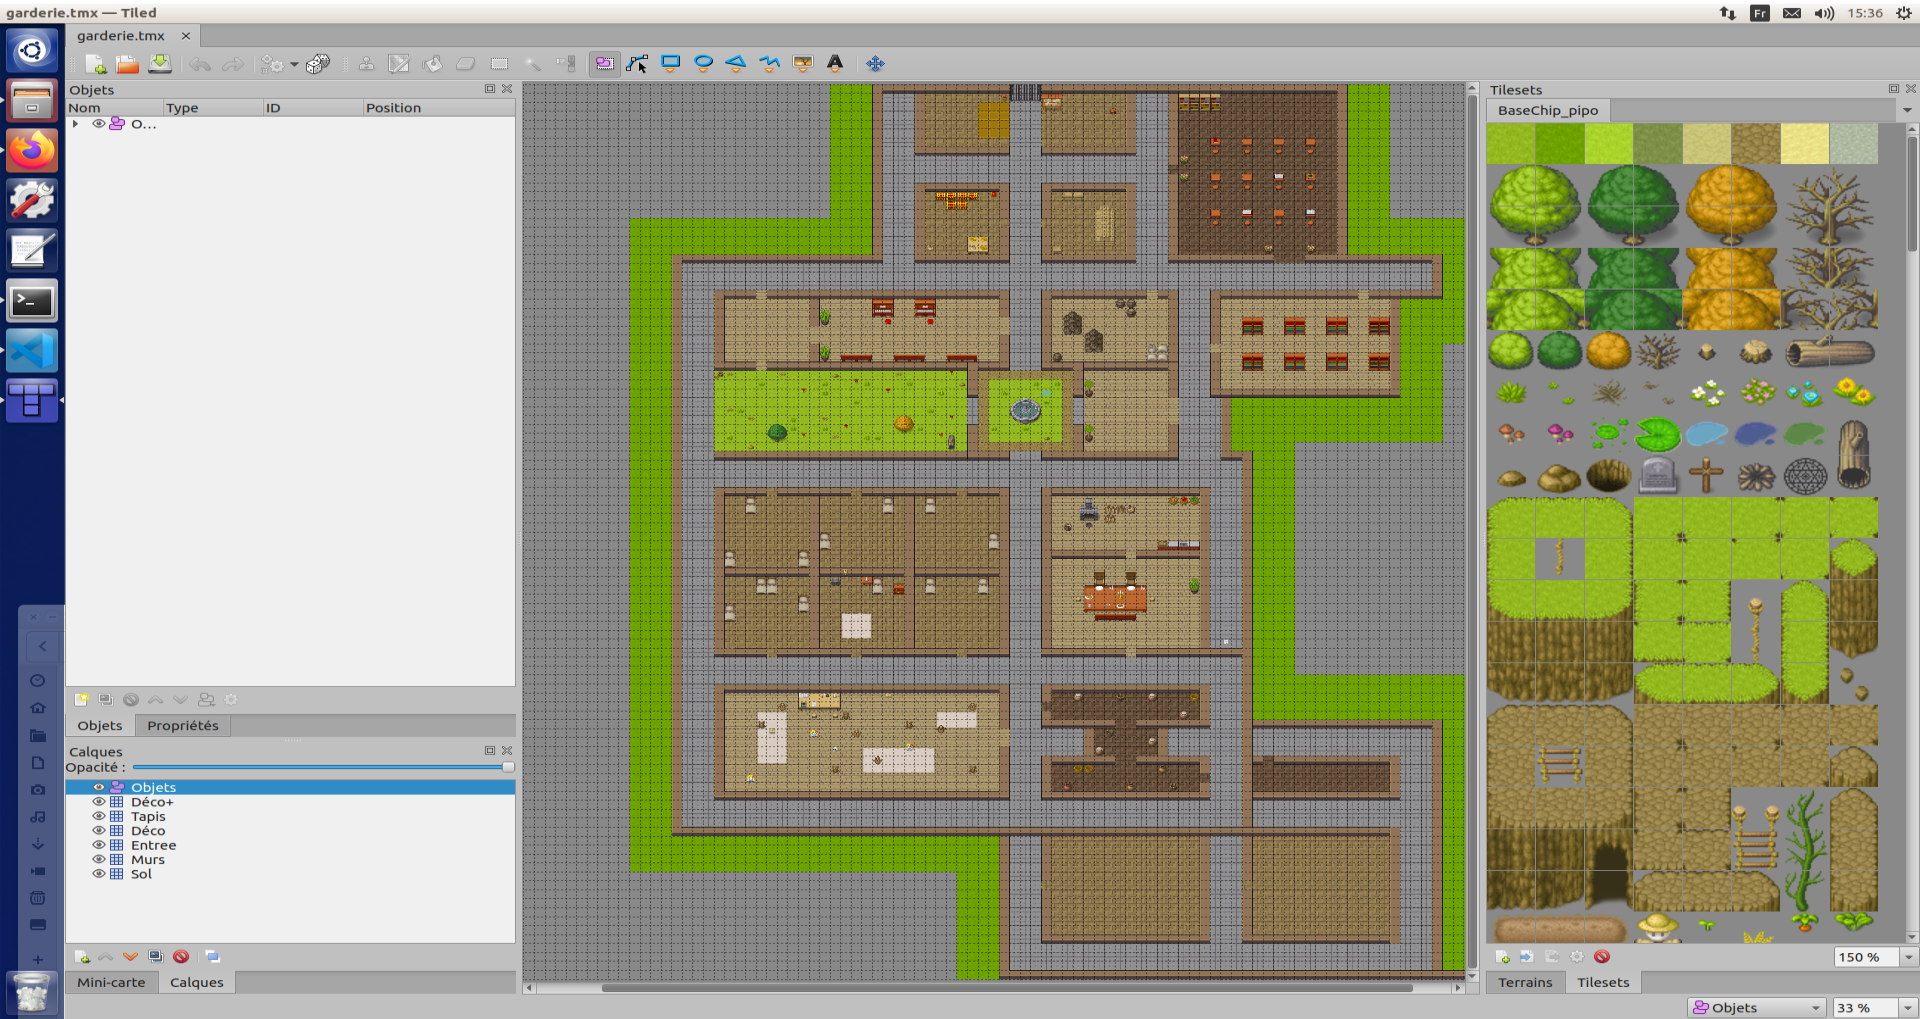
\includegraphics[scale=0.22]{images/map_entiere.png}
    \caption{Carte dans Tiled}
    \label{map_entiere}
    \end{center}
\end{figure}
On peut voir sur la droite une partie du \textbf{Tileset} permettant de mettre une tuile dans les cases de notre carte.
\newpage 
Pour implémenter cette carte dans notre jeu, nous avons crée une classe \textbf{Map} dans laquelle nous supplantons les fonctions \textbf{visitTileLayer} et \textbf{visitObjectLayer}. En effet, notre carte est divisé en layers (couche) et dans notre carte nous avons différents layers.
\begin{figure}[ht]
    \begin{center}
    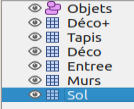
\includegraphics[scale=1]{images/Layers.png}
    \caption{Différents layers}
    \label{layers}
    \end{center}
\end{figure}
Divisé les différentes parties de la carte est non seulement pratique pour sa conception, mais cela permet aux deux fonctions de parser (analyser) chacun des layers et d'agir en fonction de celui-ci. Dans la fonction \textbf{visitTileLayer}, on tente de récupérer la texture de la tile lors du parcours de l'ensemble des tiles présentes dans le layer et dans la carte. Ces différents layers permettent de \og mixer\fg des tiles, par exemple si on souhaite poser une tasse sur la même tuile qu'une table, on peut grâce à un layer différent de celui de la table.\\
Par exemple pour gérer les collisions, nous nous sommes dit que nous avions besoin de collisions avec les murs de la carte et de certains objets décoratifs. Nous avons donc dans notre classe \textbf{Physics} supplanté \textbf{visitTileLayer} et \textbf{visitObjectLayer} pour parser les layers et ajouter une hitbox pour chacun des murs présents de le layer \og Murs\fg.
Nous avons fait de même pour le layer \og Déco\fg qui représente les différentes décorations placées sur la carte. Il existe un layer \og Objets\fg qui un est un peu différent des autres. C'est un calque d'objets contrairement aux autres qui sont des calques de tuiles. Cela permet de placer des sprites ou tuiles là où nous souhaitons sans être obligé d'être sur une grille contrairement à un calque de tuiles. 
\begin{figure}[ht]
    \begin{center}
    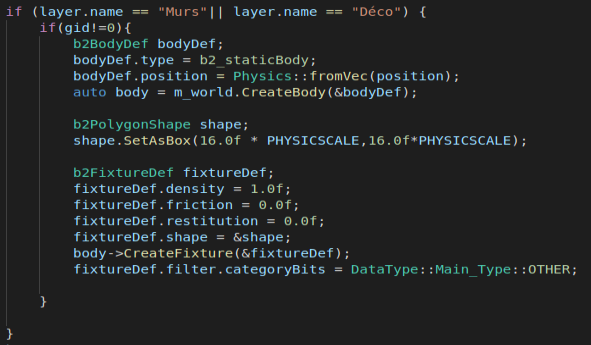
\includegraphics[scale=0.61]{images/physics_tile_layer.png}
    \caption{Différents layers}
    \label{physics_tile_layer}
    \end{center}
\end{figure}

\subsubsection{Gestion des bonus}

\subsubsection{Gestion de la carte}

\subsubsection{Gestion du son}
Il existe dans K.G.B. une musique de fond afin d'ajouter une ambiance sonore. Nous avons ajouter des bruitages, un pour les bruits de pas du bébé, un pour ramasser un bonus, un pour le bonus de rapidité et un pour le bonus d'invisibilité. Les dialogues de l'introduction du jeu sont doublés par Mathieu. 
Pour implémenter le son, nous avons utilisé la bibliothèque audio de SFML.
\begin{figure}[ht]
    \begin{center}
    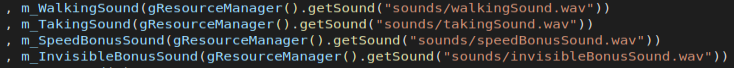
\includegraphics[scale=0.61]{images/baby_sounds.png}
    \caption{Bruitages implémentés}
    \label{baby_sounds}
    \end{center}
\end{figure}
Pour se faire, nous stockons les différents bruitages. Il nous suffit ensuite de faire par exemple : \texttt{\textbf{m\_TakingSound.play()}} pour jouer le son et \texttt{\textbf{m\_TakingSound.stop()}} pour arrêter le son. L'utilisation de SFML est très simple et intuitive. Nous appelons donc ces fonctions principalement au moment où le bébé est en mouvement et quand il ramasse ou encore utilise un bonus.

\subsubsection{Mode \og Debug\fg}
Pour vérifier que les hitbox des différents personnages soient bien placés, autrement dit qu'elles épousent la forme du personnage ou du mur, nous utilisons un mode Debug utilisable avec la touche \textbf{F10}. Ce mode Debug affiche pour chaque Fixture la forme de la hitbox de celle-ci. Par exemple celle du bébé est une hitbox carré, alors on va afficher un carré avec les tailles correspondantes.

\newpage

\subsection{Déroulement du jeu}
La boucle du jeu se compose de plusieurs phase représenté par un état:
    \begin{itemize}
        \item \textbf{INTRO} Lançant l'introduction du jeu.
        \item \textbf{PLAYING} Débutant le jeu.
        \item \textbf{VICTORY} Affichant l'écran de victoire.
        \item \textbf{GAMEOVER} Affichant l'écran de game over.
    \end{itemize}\bigbreak
Quand l'état courant est INTRO la fenêtre affiche tour à tour les différentes images ainsi que le texte et le son associé de manière à présenter le jeu à l'utilisateur. Le joueur peut décider à tout moment de passer la cinématique à l'aide du bouton p et peut passer à l'image suivante en appuyant sur espace. Tout au long de l'introduction les actions de jeu sont désactivées.\bigbreak
Durant la phase de jeu les actions qui lui sont associées sont actives et celle de l'introduction sont alors désactivées à leur tour. L'\textbf{ATH} (Affichage Tête-Haute ou HUD en anglais) est alors affiché de manière à ce que le joueur puisse se renseigner sur les commandes ou sur son nombre de bonus.
À chaque update la vélocité du bébé est mise à jour en fonction des touches qui ont été pressées par le joueur. Enfin toutes les entités sont mises à jour à travers une fonction update répartie dans chacune des classes.\bigbreak
Finalement les états VICTORY et GAMEOVER affichent respectivement les écrans de victoire et de game over suivant si le joueur à réussi ou non à s'échapper. Durant ces phases les actions de jeu sont de nouveau désactivées et la fenêtre se ferme automatiquement au bout de quelques secondes. 

\section{Gestion du projet}

\subsection{Organisation}
Afin de gérer au mieux le travail de chacun, nous utilisons un gestionnaire de version bien connu : \textbf{GitHub}.
Notre dépôt est disponible à l'adresse suivante : \texttt{https://github.com/JeanPOULET/ProjetTutore}.
Nous utilisons \textbf{Discord} qui est un logiciel de messagerie instantanée et peut servir pour de communications vocales. Dans l'idéal, une fois que quelqu'un avait fini un élément qu'il voulait implémenter il en parlait directement dans notre salon Discord dédié au projet. De même quand quelqu'un avait un problème, ou était bloqué dans ce qu'il souhaitait faire il en parlait aux autres.


\subsection{Problèmes/défis rencontrés}
Nous avons eu quelques soucis pour démarrer notre projet. En effet, le projet devait débuter en novembre. Nous avons pris un certain temps à nous lancer dans le projet. Peu de temps après le commencement, nous avons tenté d'installer Box2D, ce qui malheureusement nous a pris beaucoup de temps car nous n'avions pas la bonne librairie. Ce qui nous a assez découragé au début. Cependant une fois ce problème résolu, nous avons eu quelques soucis de versions qui ne nous permettaient de compiler (problèmes pour Jérémy et Mathieu). Nous avons du passer sur Ubuntu 18.04 au lieu de 16.04. Après la mise à jour, Jérémy a eu un problème avec openGL. En effet, il a du changer le contrôleur graphique de sa VirtualBox pour que la fenêtre du jeu fonctionne correctement. A part ces soucis que nous avions au début, nous n'avons pas eu de problèmes excessifs. Pour les difficultés que nous avons rencontrées pendant le développement, nous avons pu en discuter et trouver des solutions avec notre tuteur de projet.

\subsection{\'Evolutions possibles}
Au début du développement du jeu nous avons pensé à plusieurs idées qu'y n'ont pas été implémentées faute de temps. Nous avions d'abord pensé à faire un jeu dans lequel le joueur aurait pu diriger plusieurs personnages à l'instar du jeu : \textit{Commandos, derrière les lignes ennemis}, pensant à demander une co-gestion de ceux-ci afin de réaliser divers objectifs et notamment de les réunir tous pour pouvoir ouvrir la porte de sortie. De même le bébé aurait pu \og neutraliser \fg les ennemies en tirant une couche dessus afin de les étourdir durant un temps limité. Nous avons implémenter une couche bonus permettant de récupérer des munitions.\bigbreak
Enfin nous aurions pu augmenter le nombre d'objectifs (déverrouiller une porte, trouver un code, etc.) mais il aurait fallu pour cela agrandir la carte ou varié le type d'objectifs afin de ne pas faire d'objectifs trop redondant pour ne pas ennuyer le joueur.



\section{Conclusion}

\section{Annexes}
\subsection{Organigramme}
\subsection{Sources}
\subsection{Glossaire}


\end{document}
